\documentclass[preprint,11pt,a4paper,times,doubleblind]{elsarticle}
\usepackage{amsmath,amssymb,bm}
\usepackage{graphicx}
\usepackage{booktabs}
\usepackage{array}
\usepackage{tabularx}
\usepackage[font=small,labelfont=bf]{caption}
\usepackage{microtype}
\usepackage{xr}
\externaldocument{manuscript_submission}
\usepackage[hidelinks]{hyperref}
\graphicspath{{figs/}}
\setlength{\parskip}{2pt}
\renewcommand{\thetable}{S\arabic{table}}
\renewcommand{\thefigure}{S\arabic{figure}}
\journal{International Journal of Heat and Mass Transfer}

\begin{document}
\begin{frontmatter}
\title{Supplementary material for:\\
Temperature-contrast scaling of the Boussinesq--compressible gap for single-contrast
convection data reuse}
\author[a]{}
\address[a]{}
\hypersetup{pdfauthor={Anonymous}}
\begin{abstract}
This supplement collects the material that supports the main text but is not needed in the flow of
its argument: the asymptotic predictions and their numerical confirmation, the two-parameter fits,
the exact single-$\varepsilon$ transfer matrix, the learning curve, the public-data splits, the
prefactor--velocity law, the pressure-alignment protocol, the shape-stability and data-set tables,
the wall-heat-transfer tables, the full three-dimensional fits, and the mesh- and noise-audit
details. Table and section numbers in cross-references refer to the main text.
\end{abstract}
\end{frontmatter}

The runs behind every number in the main text are: 600 main solutions
(\path{run_batch.sh}), 100 paired (\path{run_paired.sh}), 27 at
$\varepsilon\to0$ (\path{run_eps0.sh}), 104 at $Pr=4.38$ (\path{run_water.sh});
\path{run_cpu_queue.sh} adds the 2:1 geometry and the tight-tolerance reruns.

\begin{table}[htbp]
\centering
\small
\caption{The five testable consequences of the expansion and their measured values.}
\label{tab:predictions}
\begin{tabular}{@{}p{3.2cm}p{9.0cm}@{}}
\toprule
prediction & measurement\\
\midrule
$R\to0$ as $\varepsilon\to0$ & intercept $+0.0003\pm0.0047$ ($u_x$); $0.06\sigma$ from zero\\
$R\propto\varepsilon$ & $m=1.023\pm0.018$ / $0.995\pm0.019$ / $1.009\pm0.015$
($u_x/u_y/p$), window-averaged over the two decades; the residual is the $\varepsilon^2$ term
(Sec.~\ref{sec:law})\\
the shape of $D$ does not rotate with $\varepsilon$ & $\cos(D(\varepsilon),D(1.2))=0.95$--$1.00$,
four channels $\times$ five values of $\varepsilon$\\
$\nabla\cdot\bm u_1=\nabla\cdot(\theta_0\bm u_0)$ & $\mathrm{div}(Y)$ vs
$\varepsilon\nabla\cdot(\theta\bm u_X)$: cosine $+0.994$ for $\varepsilon<0.6$, $+0.965$ overall,
amplitudes $2.26\times10^{-2}$ vs $2.10\times10^{-2}$\\
the expansion converges fast & per configuration, $\varepsilon^1$ alone carries 86\% of the
correction energy, $\varepsilon^1+\varepsilon^2$ carries 99.0\%, $\varepsilon^3$ carries 99.9\%\\
\bottomrule
\end{tabular}
\end{table}

\begin{table}[htbp]
\centering
\small
\caption{Two-parameter refinement, $R=A\varepsilon^mRa^q$. The $Ra$ trend for $u_y$ and $\theta$
reproduces in the 2:1 geometry.}
\label{tab:two-param}
\begin{tabular}{@{}lcc@{}}
\toprule
channel & unit cavity ($n=600$) $m$ / $q$ / $R^2$ & aspect 2:1 ($n=104$) $m$ / $q$ / $R^2$\\
\midrule
$u_x$ & $1.081$ / $+0.003\pm0.006$ / $0.74$ & $1.071$ / $-0.143\pm0.019$ / $0.71$\\
$u_y$ & $1.016$ / $-0.083\pm0.005$ / $0.77$ & $1.146$ / $-0.077\pm0.019$ / $0.69$\\
$\theta$ & $1.120$ / $+0.514\pm0.015$ / $0.72$ & $0.989$ / $+0.447\pm0.045$ / $0.55$\\
$p$ & $1.127$ / $-0.029\pm0.005$ / $0.83$ & $1.057$ / $-0.154\pm0.017$ / $0.74$\\
\bottomrule
\end{tabular}
\end{table}

\begin{table}[htbp]
\centering
\small
\caption{Exact transfer error $R(u_x)$ when a field computed at one $\varepsilon$ (rows) is
applied at another (columns).}
\label{tab:transfer-matrix}
\begin{tabular}{@{}lccccc@{}}
\toprule
$R(u_x)$ taken from $\downarrow$ / applied at $\to$ & 0.4 & 0.8 & 1.2 & 1.6 & 1.9\\
\midrule
$\varepsilon=0.4$ & 0 & 0.067 & 0.143 & 0.235 & 0.353\\
$\varepsilon=0.8$ & 0.068 & 0 & 0.078 & 0.183 & 0.305\\
$\varepsilon=1.2$ & 0.149 & 0.081 & 0 & 0.110 & 0.243\\
$\varepsilon=1.6$ & 0.265 & 0.199 & 0.112 & 0 & 0.140\\
$\varepsilon=1.9$ & 0.402 & 0.328 & 0.251 & 0.142 & 0\\
\bottomrule
\end{tabular}
\end{table}

\begin{table}[htbp]
\centering
\footnotesize
\setlength{\tabcolsep}{4pt}
\caption{Learning curve on the fixed interpolation test set (200 samples), mean of three seeds.
Entries are $u_x/u_y/\theta/p$. P3 keeps $\varepsilon$ outside the network entirely.}
\label{tab:learning}
\begin{tabular}{@{}c p{5.0cm}p{5.0cm}@{}}
\toprule
$n$ & B: $\varepsilon$ as input & P3: predict $P(X)$, $\varepsilon$ outside\\
\midrule
0 (do nothing) & 0.2203/0.2683/0.0381/0.2386 & same\\
50 & 0.1831/0.1946/0.0269/0.1838 & \textbf{0.1308/0.1364/0.0195/0.1501}\\
100 & 0.1280/0.1422/0.0199/0.1348 & \textbf{0.0990/0.1022/0.0136/0.1150}\\
200 & 0.0974/0.1070/0.0147/0.0998 & \textbf{0.0827/0.0866/0.0114}/0.1005\\
400 & \textbf{0.0674/0.0714}/0.0097/\textbf{0.0672} & 0.0735/0.0743/0.0093/0.0896\\
\bottomrule
\end{tabular}
\end{table}

\begin{table}[htbp]
\centering
\small
\caption{Median relative correction on all five public splits, at $\varepsilon\equiv1.2$.}
\label{tab:splits}
\begin{tabular}{@{}lccccc@{}}
\toprule
split & $n$ & $u_x$ & $u_y$ & $\theta$ & $p$\\
\midrule
train (random walls) & 4000 & 0.1797 & 0.2435 & 0.0228 & 0.1858\\
test\_in\_distribution & 200 & 0.1822 & 0.2388 & 0.0220 & 0.1863\\
test\_ood (harder wall dials) & 200 & 0.1567 & 0.2157 & 0.0214 & 0.1671\\
train\_legacy (classical cavity) & 5000 & 0.2988 & 0.3362 & 0.0926 & 0.1989\\
test\_legacy (classical cavity) & 200 & 0.2984 & 0.3390 & 0.0836 & 0.1983\\
\bottomrule
\end{tabular}
\end{table}

\begin{table}[htbp]
\centering
\small
\caption{The $\theta$-channel prefactor is the flow strength: $R_\theta/\varepsilon=c\hat u^a$ on
six data sets from two independent generators.}
\label{tab:uhat}
\begin{tabular}{@{}lccc@{}}
\toprule
data set & $n$ & $R_\theta/\varepsilon=c\hat u^a$ & $R^2$\\
\midrule
ours, random walls, $Pr=0.71$ & 600 & $a=1.864\pm0.026$, $c=0.544$ & 0.90\\
public train, random walls & 4000 & $a=1.902\pm0.010$, $c=0.602$ & 0.91\\
public test\_in\_distribution & 200 & $a=1.977\pm0.041$, $c=0.691$ & 0.92\\
public test\_ood & 200 & $a=1.931\pm0.041$, $c=0.561$ & 0.92\\
public train\_legacy, classical cavity & 5000 & $a=2.360\pm0.002$, $c=2.063$ & \textbf{0.995}\\
public test\_legacy, classical cavity & 200 & $a=2.368\pm0.011$, $c=2.095$ & \textbf{0.996}\\
\bottomrule
\end{tabular}
\end{table}

\begin{table}[htbp]
\centering
\footnotesize
\setlength{\tabcolsep}{4pt}
\caption{Scripts and the results they produce.}
\label{tab:scripts}
\resizebox{\textwidth}{!}{%
\begin{tabular}{@{}>{\raggedright\arraybackslash}p{5.2cm}>{\raggedright\arraybackslash}p{10.4cm}@{}}
\toprule
script & what it produces\\
\midrule
\path{exp_eps_law.py} & the 627-sample law (Sec.~\ref{sec:law})\\
\path{exp_grid128.py} & the $64^2$ vs $128^2$ mesh check at $Ra=10^4$ and $Ra=10^6$
(Sec.~\ref{sec:law})\\
\path{repack_p_fixed.py} & the corrected pressure channel (Sec.~\ref{sec:pressure})\\
\path{exp_paired_final.py} & the $\varepsilon$-blind floor and shape invariance
(Sec.~\ref{sec:floor})\\
\path{exp_modes.py} & the $\varepsilon^k$ mode expansion (Sec.~\ref{sec:theory})\\
\path{exp_chi.py} & the $\chi$ explanation for $\theta$ (Sec.~\ref{sec:law})\\
\texttt{harness.py}, \path{exp_ml_final.py} & the unified surrogate ablation: A/B/P1/P2/P3,
three seeds (Secs.~\ref{sec:baselines}--\ref{sec:learning})\\
\path{fno_lib.py}, \path{exp_fno_final.py} & the FNO baseline under the same protocol
(Sec.~\ref{sec:prior})\\
\path{exp_lc_final.py} & learning curves (Sec.~\ref{sec:learning})\\
\path{exp_pod.py} & the POD-ROM / linear-surrogate baselines (Sec.~\ref{sec:baselines})\\
\path{exp_direct_linear.py}, \path{exp_direct_batch.py} & the direct solution of the linearised $O(\varepsilon)$ system on all 20 configurations (Sec.~\ref{sec:baselines})\\
\path{exp_direct_eps0.py} & the same one-Newton-step solve on the 27 low-contrast samples (Sec.~\ref{sec:baselines})\\
\path{exp_heldout_loweps.py}, \path{run_loweps.sh} & the 38 held-out solutions at $\varepsilon=0.1,0.2$ and the extrapolated-$P$ check (Sec.~\ref{sec:baselines})\\
\path{exp_direct_low.py}, \path{exp_fixed_flow_eps.py} & one-Newton-step solves at $\varepsilon=0.1,0.2$ on the paired flows and the fixed-flow $\varepsilon$-drift (Sec.~\ref{sec:baselines})\\
\path{exp_cluster_boot.py} & family-cluster bootstrap of the exponent (Sec.~\ref{sec:law})\\
\path{exp_public_transfer.py} & external validation and transfer
(Secs.~\ref{sec:public}--\ref{sec:transfer})\\
\path{exp_fair_scaling.py} & fair baseline: plain model trained at $\varepsilon_0$ and
rescaled by $\varepsilon/\varepsilon_0$ (Table 3)\\
\path{exp_aspect2.py} & the 2:1 geometry (Sec.~\ref{sec:aspect})\\
\path{exp_tight.py}, \path{verify_noise.py},\newline \path{exp_final_numbers.py} & noise control
and timing (Secs.~\ref{sec:noise}--\ref{sec:cost})\\
\path{exp_water.py} & the strictly paired $Pr=4.38$ fluid study (Sec.~\ref{sec:water})\\
\path{exp_perturbation.py} & the first-order perturbation baseline on the $\varepsilon$ scan
(Sec.~\ref{sec:baselines})\\
\path{exp_linear_response.py} & the linear-response and secant baselines from the paired scan
(Sec.~\ref{sec:baselines})\\
\path{exp_second_order.py} & the two-term $P+\varepsilon Q$ fit from the paired scan
(Supplementary Sec.~S10)\\
\path{exp_nu_clean_summary.py} & the isothermal-sidewall $Nu$ statistics and the
denominator audit (Sec.~\ref{sec:nu})\\
\path{exp_nu_grid.py}, \path{exp_nu_grid_ra1e6.py}, \path{exp_nu_grid_ra1e5.py} & the
$64^2$ versus $128^2$ wall-flux check (Supplementary Sec.~S10)\\
\path{exp_public_nu.py}, \path{exp_flux_loss.py}, \path{exp_flux_stencil.py} & wall heat transfer of the
public-data surrogate, with and without the wall-flux training penalty, and the cross-stencil check
(Sec.~\ref{sec:nu})\\
\path{exp_field_vs_nu.py}, \path{exp_seed_sweep.py}, \path{exp_own_seed_sweep.py} & per-sample
field-versus-$Nu$ statistics, the source-normalised multi-seed transfer, and the within-family
replication (Sec.~\ref{sec:headline})\\
\path{make_fig_field_nu.py}, \path{make_fig_nu_eps_ra.py} & the field--$Nu$ scatter and the
$\varepsilon$/$Ra$ heat-transfer figure (Secs.~\ref{sec:headline}--\ref{sec:nu})\\
\path{exp_film.py} & the FiLM-conditioned baseline (Sec.~\ref{sec:prior})\\
\path{exp_3d_law.py},\newline \path{exp_3d_exp.py},\newline \path{exp_2d_ra_window.py},\newline \path{merge_3d.py},\newline \path{exp_3d_summary.py},\newline \path{make_fig9.py},\newline \path{exp_3d_rom_eps.py} & the thirty-three-sample three-dimensional check at three Rayleigh numbers and the POD-ROM baseline (Sec.~\ref{sec:3d})\\
\path{verify_conventions.py} & the 38\,400-value convention audit against the published
\texttt{relL2} columns (Sec.~\ref{sec:public})\\
\path{exp_public_splits.py},\newline \path{exp_legacy5000.py}, \path{exp_uhat_law.py} & the
five public splits and the $\hat u$ law (Sec.~\ref{sec:public})\\
\path{exp_transfer_uhat.py} & the $\hat u$ transfer criterion on the public splits
(Sec.~\ref{sec:transfer})\\
\path{audit_v2.py} & robustness checks: $m$ vs fitting window,
$\kappa$, pressure-pair conventions, $\hat u$ medians, the 2:1 $\sigma$ distances\\
\path{make_figs.py}, \path{make_figs2.py} & every figure, from the JSON results\\
\path{make_tables.py} & regenerates every table from the JSON results\\
\bottomrule
\end{tabular}}
\end{table}

\section*{S1 A POD-ROM check of the prior}
The fifteen samples at $Ra=10^4$ (described in Sec.~S9) also support a linear surrogate check. We train a POD-ROM with at most four modes on three flows and four
contrasts (twelve samples) and test on the held-out contrast (three samples),
repeating for each of the five contrasts. The plain ROM predicts $D$ from
$[1,\varepsilon,\bm c_X]$, where $\bm c_X$ are at most four POD coefficients of the
Boussinesq field; the prior ROM predicts $P=D/\varepsilon$ from
$[1,\bm c_X]$ and multiplies by $\varepsilon$ outside. At most four modes are used,
fewer than the twelve training samples. Averaged over the five held-out contrasts,
the prior lowers the relative error in every channel (Table~\ref{tab:3drom}):
$u_x$ from 0.168 to 0.081, $u_y$ from 0.190 to 0.150, $\theta$ from 0.034 to
0.027 and $p$ from 0.163 to 0.098. The gain is largest at $\varepsilon=0.2$ and
0.4 ($14\times$ and $5\times$ in $u_x$) and is not uniform: at $\varepsilon=1.2$ the
$\varepsilon$-aware plain ROM is better in all four channels. We read this as a
check that the factorisation remains useful in three dimensions at small
contrast, not as a claim of uniform superiority.


\begin{table}[htbp]
\centering
\small
\caption{Three-dimensional POD-ROM check on the fifteen paired samples at $Ra=10^4$.
Leave-one-contrast-out: train on three flows $\times$ four $\varepsilon$
(twelve samples), test on the held-out $\varepsilon$ (three samples), repeated
for the five contrasts. Entries are mean relative $L_2$ errors over the five
folds (mean $\pm$ s.d.); the ROM uses at most four POD modes and ridge regression
($\lambda=10^{-4}$). The gain is the plain-ROM error divided by the prior-ROM error.}
\label{tab:3drom}
\begin{tabular}{@{}lcccc@{}}
\toprule
channel & do nothing & plain ROM & prior ROM & gain\\
\midrule
$u_x$ & 0.1934$\pm$0.132 & 0.1676$\pm$0.071 & 0.0807$\pm$0.061 & 2.08\\
$u_y$ & 0.1880$\pm$0.127 & 0.1901$\pm$0.046 & 0.1497$\pm$0.100 & 1.27\\
$\theta$ & 0.0362$\pm$0.025 & 0.0338$\pm$0.008 & 0.0270$\pm$0.019 & 1.25\\
$p$ & 0.1617$\pm$0.117 & 0.1634$\pm$0.065 & 0.0980$\pm$0.077 & 1.67\\
\bottomrule
\end{tabular}
\end{table}

\section*{S2 The Prandtl-number pair}
Same configuration, same $\varepsilon$, only $Pr$ changed: 104 paired samples at
$Pr=0.71$ and $Pr=4.38$. The table gives the fits, the figure the paired comparison.

\begin{table}[htbp]
\centering
\footnotesize
\setlength{\tabcolsep}{3pt}
\caption{The fluid axis: 104 strictly paired configurations at $Pr=0.71$ and $Pr=4.38$ (same seed
stream, same $Ra$ and $\varepsilon$). Both columns are fitted on the same 104 configurations over
their full $\varepsilon\in[0.21,1.89]$ range; the exponents are steeper than the full-window
values of Table~\ref{tab:law} because the sample subset differs, and the two are not directly
comparable. The exponent agrees between the two fluids within 1.5\%, the paired median ratio of $R$ is
0.95--1.01, and the fitted prefactors move by 3.3\% ($u_x$), 0.2\% ($u_y$), 1.2\% ($\theta$) and
6.1\% ($p$).}
\label{tab:water}
\begin{tabular}{@{}lcccc@{}}
\toprule
channel & $A$, $Pr=0.71$ & $A$, $Pr=4.38$ & $m$, $Pr=0.71$ & $m$, $Pr=4.38$\\
\midrule
$u_x$ & 0.1448 & 0.1496 & $1.157$ & $1.150$\\
$u_y$ & 0.1981 & 0.1985 & $1.047$ & $1.049$\\
$\theta$ & 0.0081 & 0.0082 & $1.668$ & $1.686$\\
$p$ & 0.1519 & 0.1426 & $1.109$ & $1.124$\\
\bottomrule
\end{tabular}
\end{table}

\begin{figure}[htbp]
\centering
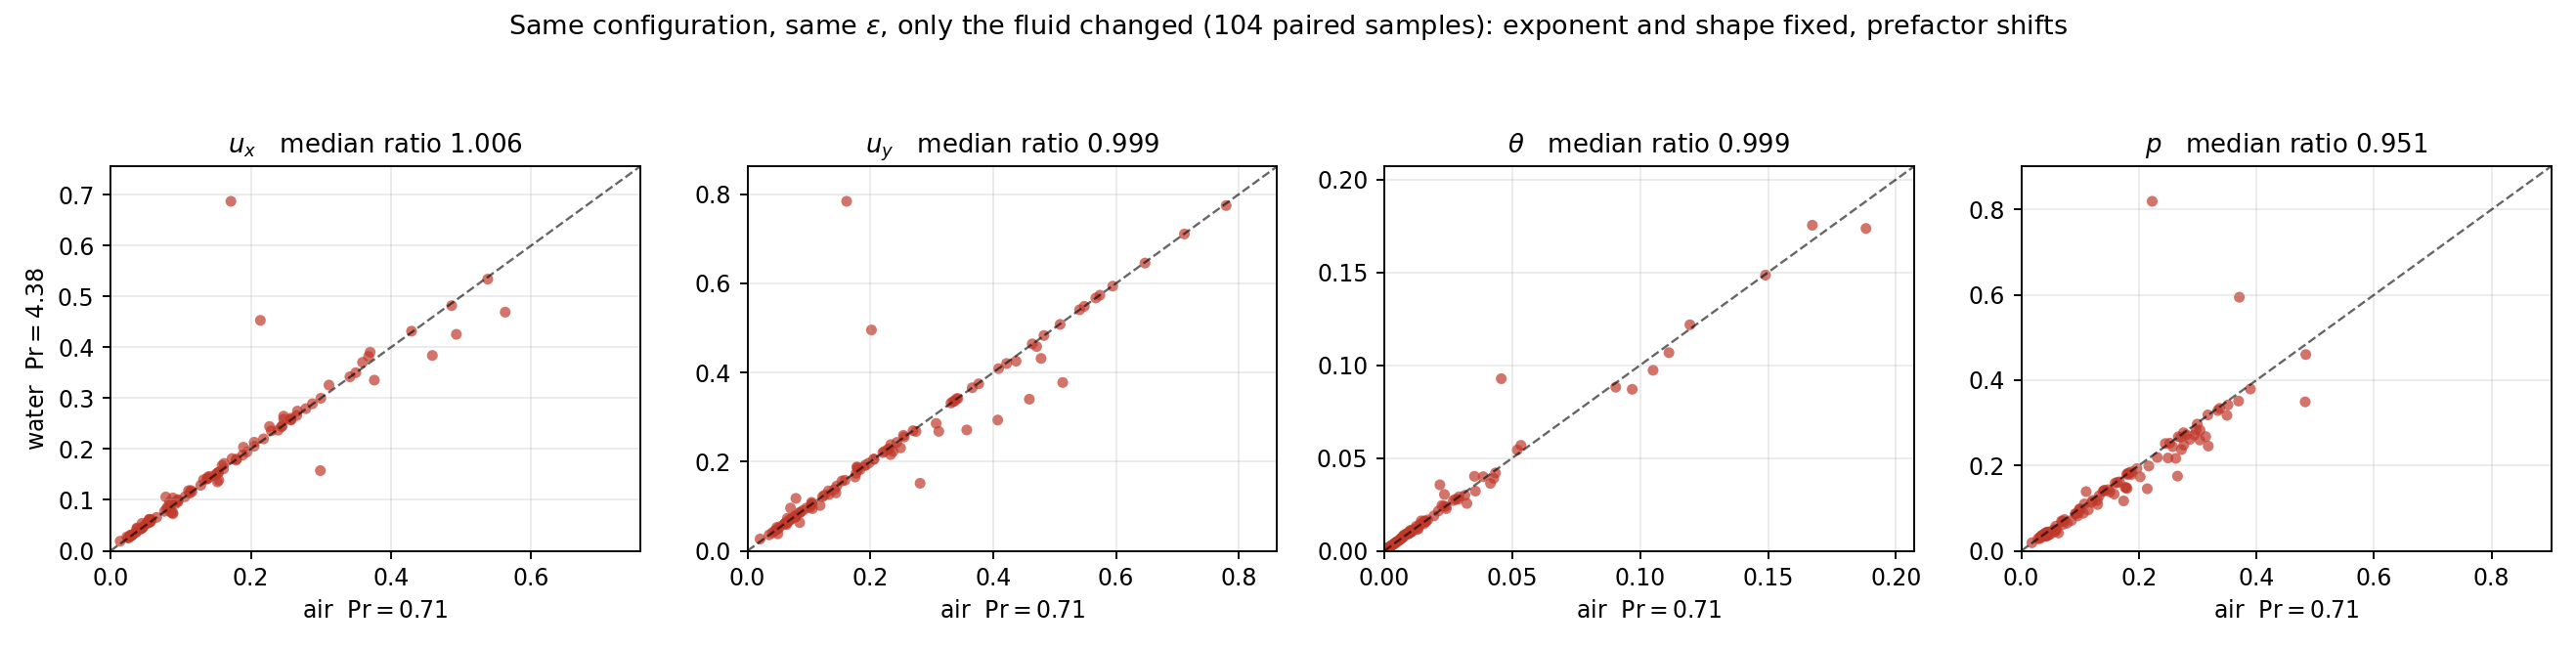
\includegraphics[width=0.96\textwidth]{fig8_water.png}
\caption{Same configuration, same $\varepsilon$, only the Prandtl number changed: $Pr=0.71$ against
$Pr=4.38$, 104 paired samples. The panel labels follow the original run names; both runs use the
same equation of state and the same dimensionless transport model; only $Pr$ (and hence the thermal
diffusivity at fixed $Ra$) differs.}
\label{fig:water}
\end{figure}

\section*{S3 Cost and speed-up}
Wall-clock timings behind the speed-up numbers in the main text.

\begin{table}[htbp]
\centering
\small
\caption{Wall-clock cost, $64^2$ mesh. Solver rows use eight CPU threads; the surrogate runs on
an RTX 4060 Laptop GPU (batch 1) or one CPU thread. The two members are timed separately over the
600 samples; the rows below them are surrogate timings or totals derived from the measured medians.
The 100-sample scan rows use that scan's own timings: the component medians are 16.0\,s
(Boussinesq) and 37.5\,s (compressible), while the median of their per-pair sum is 55.8\,s;
medians are not additive.}
\label{tab:scost}
\begin{tabular}{@{}lcccc@{}}
\toprule
quantity & median & mean & p90 & max\\
\midrule
paired solve, 600 samples & 33.9\,s & 38.0\,s & 59.9\,s & 510\,s\\
Boussinesq member alone & 11.7\,s & 13.1\,s & 21.7\,s & ---\\
compressible member alone & 22.3\,s & 25.0\,s & 37.3\,s & ---\\
paired solve, 100-sample $\varepsilon$ scan (per sample) & 55.8\,s & 67.7\,s & 136\,s & 202\,s\\
surrogate, GPU, batch 1 & 6.3\,ms & & &\\
surrogate, GPU, batch 256 & 0.49\,ms/sample & & &\\
surrogate, CPU, 1 thread & 14.0\,ms & & &\\
end-to-end pair (Boussinesq + surrogate) & 11.7\,s & & &\\
one flow, 100 contrasts (scan timing) & 16.6\,s & & &\\
20-flow $\times$ 5-contrast scan, surrogate total & 321\,s & & &\\
\bottomrule
\end{tabular}
\end{table}

\section*{S4 The pressure channel: raw and aligned statistics}
\label{sec:pressure-supp}

The two members store pressure in different conventions. The compressible raw pressure carries a
hydrostatic ramp $12\times$ larger than its dynamic part, and the two weak forms use opposite
sign conventions. Comparing raw pressures therefore measures the conventions rather than the flow:
the per-sample median of $|X_p|/|Y_p|$ is $0.065$, that of $\cos(X_p,Y_p)$ is $-0.105$, and the
$p$-channel ``law'' collapses to a constant ($R_p\approx1.0$). We align the members with the
protocol used by the public data set---subtract the mean, remove a least-squares linear-in-$y$ fit,
and flip the sign of the Boussinesq member. Under the same median convention the aligned pair gives
$0.960$ and $\cos=+0.991$, against $0.929$ and $+0.986$ for the public training set, so the two
pairings agree to within $3.5\%$. The channel then follows the same law as the velocities
($A=0.148$, $m=1.009$). All $p$-channel numbers in the paper use this gauge. Pressure is
gauge-dependent: the exponent is a statement about this fixed post-processing gauge, not a
gauge-invariant law.

\section*{S5 Shape stability of the correction}
The amplitude changes with contrast; the shape does not. Over the 20 paired configurations the
median cosine similarity between $D(\varepsilon)$ and $D(1.2)$ stays above $0.952$ for
$\varepsilon=0.4$--$1.9$, so a scalar amplitude carries the contrast dependence.

\begin{table}[htbp]
\centering
\small
\caption{Cosine similarity between the correction field $D(\varepsilon)$ and $D(1.2)$, median
over the 20 paired configurations. Values are ordered by $\varepsilon$.}
\label{tab:shape}
\begin{tabular}{@{}lccccc@{}}
\toprule
channel & 0.4 & 0.8 & 1.2 & 1.6 & 1.9\\
\midrule
$u_x$ & 0.978 & 0.994 & 1.000 & 0.992 & 0.974\\
$u_y$ & 0.993 & 0.998 & 1.000 & 0.996 & 0.976\\
$\theta$ & 0.991 & 0.997 & 1.000 & 0.996 & 0.982\\
$p$ & 0.964 & 0.991 & 1.000 & 0.990 & 0.952\\
\bottomrule
\end{tabular}
\end{table}

\section*{S6 Data sets}
The table lists the sets used in the main text.
\begin{table}[htbp]
\centering
\footnotesize
\setlength{\tabcolsep}{4pt}
\caption{Data sets used in this study. The public sets are from
Menglik et al.}
\label{tab:data}
\begin{tabular}{@{}p{3.0cm}c p{4.0cm}p{2.8cm}@{}}
\toprule
set & $n$ & what varies & purpose\\
\midrule
random-BC & 600 & $Ra\sim\log U[10^2,10^6]$, $\varepsilon\sim U[0.2,1.9]$, 134 wall-mode
families & calibrate the law, train surrogates\\
$\varepsilon\to0$ checks & 27 & $\varepsilon=0.02/0.05/0.10$ $\times$ $Ra=10^3/10^4/10^5$, three draws each &
anchor $R(0)=0$ (included in the fit)\\
paired & $20\times5$ & only $\varepsilon$; $Ra$ and the $\theta$ boundary stream fixed within a
configuration & $\varepsilon$-blind reference, shape invariance\\
aspect 2:1 & 104 & same law, geometry $2\times1$ & external validity\\
tight rerun & 10 & the 10 worst-converged samples, tolerance $10^{-6}\to10^{-8}$ & noise control\\
public, random walls (Menglik et al.) & $4000+2\times200$ & $\varepsilon\equiv1.2$; two
held-out splits differ in the range of the wall dials & external
validation, cross-data-set transfer\\
public, classical cavity (Menglik et al.) & $5000+200$ & constant hot/cold side walls,
adiabatic top and bottom, $\varepsilon\equiv1.2$; its 200 held-out pairs are the third split above
& external validation of the prefactor\\
$Pr=4.38$ (this work) & 104 & $Pr=4.38$; BC/$Ra$/$\varepsilon$ draws bit-identical to 104 of the
random-BC samples & test of the fluid axis\\
\bottomrule
\end{tabular}
\end{table}

\section*{S7 Wall heat transfer: pair statistics and the Rayleigh trend}
The first table gives the pair statistics at $\varepsilon=1.2$; the second gives the integral
change for the five isothermal-sidewall configurations, one at each Rayleigh number.

\begin{table}[htbp]
\centering
\footnotesize
\setlength{\tabcolsep}{4pt}
\caption{Wall heat transfer at $\varepsilon=1.2$ over the 200 classical-cavity samples of the
public data set. The local change is $\Delta Nu(y)/Nu(y)$ along the hot wall. The integral change is
the mean of the per-sample ratios at the six-point stencil, with the median and the 10--90\% range;
the ratio of the ensemble means is $+0.67\%$. The stencil range is the two- to eight-point
one-sided estimate of the wall gradient.}
\label{tab:nu}
\begin{tabular}{@{}p{4.4cm}p{2.5cm}p{5.2cm}@{}}
\toprule
quantity & value & spread over samples\\
\midrule
$Nu$, Boussinesq $X$ & 3.514 & ---\\
$Nu$, compressible $Y$ & 3.538 & ---\\
integral change $\Delta Nu/Nu$ & $+0.54\%$ & median $+0.58\%$, p10--p90 $+0.06$ to $+0.92\%$; per-sample mean $+0.35$ to $+0.62\%$ over stencils\\
local change, $L_1$ norm over the wall & $4.25\%$ & p90 $7.33\%$; unchanged for two to eight points\\
local change, pointwise & $-0.65\%$ (median) & p10--p90 $-9.1$ to $+9.8\%$\\
\bottomrule
\end{tabular}
\end{table}

\begin{table}[htbp]
\centering
\footnotesize
\setlength{\tabcolsep}{5pt}
\caption{Integral Nusselt change $\Delta Nu/Nu$ (percent) for the five isothermal-sidewall
configurations, one at each $Ra$. These are the only configurations with a positive $O(1)$
denominator at every contrast; this is the classical-cavity family, fixed before the analysis.
Random-wall families are excluded because 8 of 15 have $|Nu_X|\le1$ at $\varepsilon=1.9$. At
$Ra=10^2$ the entries are below the $0.35\%$ estimator error and are listed only for
completeness. At $Ra=10^6$ the $\varepsilon=1.2$ entry falls to $+0.44\%$ on a $256^2$ mesh and the
$\varepsilon=1.9$ entry to $-2.10\%$ on a $192^2$ mesh.}
\label{tab:nu_ra}
\begin{tabular}{@{}lccccc@{}}
\toprule
$Ra$ & $\varepsilon=0.4$ & 0.8 & 1.2 & 1.6 & 1.9\\
\midrule
$10^2$ & $-0.00$ & $+0.00$ & $+0.01$ & $+0.01$ & $-0.01$\\
$10^3$ & $+0.07$ & $+0.28$ & $+0.59$ & $+0.76$ & $-0.98$\\
$10^4$ & $+0.07$ & $+0.20$ & $+0.27$ & $-0.38$ & $-5.14$\\
$10^5$ & $+0.16$ & $+0.48$ & $+0.87$ & $+0.91$ & $-1.81$\\
$10^6$ & $+0.24$ & $+0.51$ & $+0.82$ & $+0.83$ & $-1.50$\\
\bottomrule
\end{tabular}
\end{table}

\section*{S8 Public-data splits and the theta collapse}
The release publishes three held-out splits generated by the same generator and the same solver
commit (\path{v6_freefall_20260921}, \path{raw_both_deramp} pressure convention; the OOD split
carries the later tag \path{v6_freefall_ood_20260925}): \path{test_in_distribution} (200 random-wall
pairs), \path{test_ood} (200 random-wall pairs whose vertical-wall Fourier dials lie outside the
training range) and \path{test_legacy} (200 classical-cavity pairs). The release also contains
\path{train_legacy}, 5000 classical-cavity pairs, used in the transfer experiment of the main text.
The $\theta$-channel prefactor collapses on the peak Boussinesq speed $\hat u$ across two
independent generators and two boundary-condition families.

\begin{figure}[htbp]
\centering
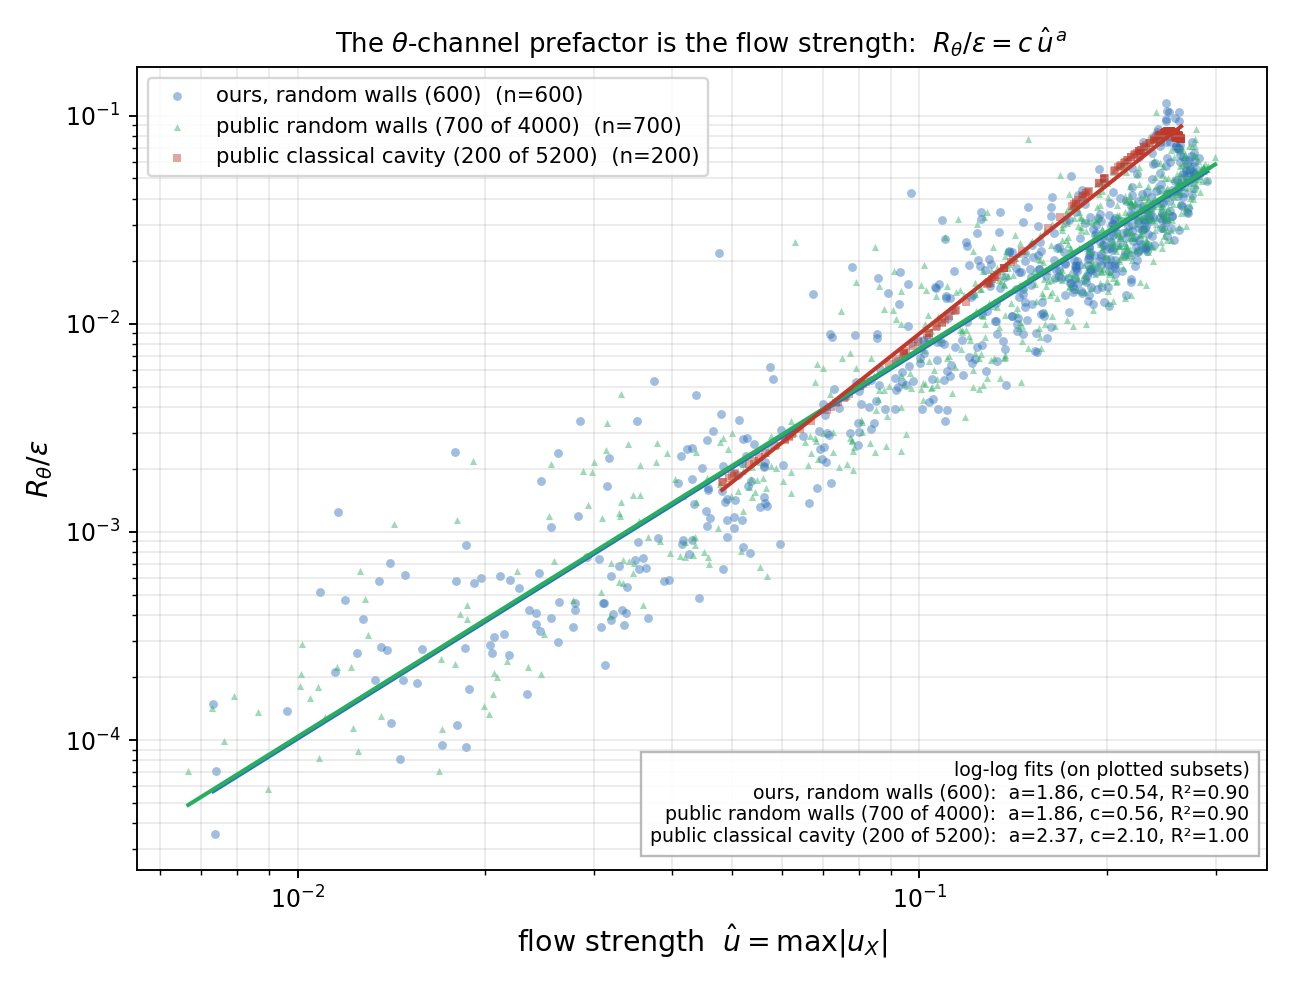
\includegraphics[width=0.78\textwidth]{fig7_theta_flow.png}
\caption{The $\theta$-channel prefactor collapses on the peak Boussinesq speed $\hat u$ across two
independent generators and two boundary-condition families.}
\label{fig:stheta}
\end{figure}

\section*{S9 A three-dimensional check}


The law is calibrated in two dimensions. To check whether the exponent survives in three, we
generated thirty-three paired steady solutions with the same generator: three wall types---a
three-cell Voronoi pair, a two-cell Voronoi pair and a constant-wall cavity---at $Ra=10^4$ over
$\varepsilon=0.2$, $0.4$, $0.8$, $1.2$ and $1.6$ (fifteen samples), and the same three wall types
at $Ra=3\times10^4$ and $Ra=10^5$ over $\varepsilon=0.4$, $1.2$ and $1.9$ (nine samples each), with $Pr=0.71$ and
$res=16$ ($33^3$ velocity nodes, $17^3$ temperature and pressure nodes). Within each set the
pairing is exact: the wall temperatures are the same seed stream scaled affinely about $T_0$, so the
low-fidelity member is the same solution up to the $\varepsilon$-blind rescaling of
Sec.~\ref{sec:blind}.
For the pressure channel we use the same fixed gauge as in two dimensions: subtract the mean,
remove a linear fit in $y$ (the gravity direction), and flip the sign; the horizontal $z$ direction
is not deramped. The $p$ exponents below are therefore fixed-gauge numbers, as in
Table~\ref{tab:law}.

Table~\ref{tab:3d} and Fig.~\ref{fig:3d} give the result. The fit is the one the two-dimensional
law takes, $R_{f,c}=A_{f,c}\varepsilon^{m_c}$: a separate prefactor for each flow and channel, and
one exponent per channel and Rayleigh number. At $Ra=10^4$ the exponents for $u_x$, $u_y$ and $p$
are $1.091\pm0.013$, $1.052\pm0.011$ and $1.141\pm0.020$ ($R^2\ge0.997$); at $Ra=3\times10^4$ they
are $1.026\pm0.066$, $1.041\pm0.063$ and $1.086\pm0.110$ ($R^2\ge0.96$); at $Ra=10^5$ they are
$1.013\pm0.060$, $1.012\pm0.052$ and $1.091\pm0.113$ ($R^2\ge0.96$). All nine lie within $0.15$
of unity. The largest difference between the two lower Rayleigh numbers is $0.065$ ($u_x$), against a
combined standard error of $0.067$; the comparison is inconclusive and does not exclude a Rayleigh
dependence of about $0.2$ over a factor of three. The $\theta$ rows, $1.130\pm0.019$ and
$1.041\pm0.081$, and $1.060\pm0.087$ at $Ra=10^5$ (the two lower-Ra difference is
$0.089\pm0.083$), are reported separately; $\theta$ does not enter the
common-exponent claim here any more than in Sec.~\ref{sec:law}.

At $Ra=10^5$ the per-flow slopes span $0.91$--$1.40$; the constant-wall pressure slope,
$1.40\pm0.22$ on three points, is the least constrained and drives the common-fit standard
error. The common fit with flow intercepts is $1.09\pm0.11$, the number quoted above.

The two lower-Ra sets also cover different windows, $0.2$--$1.6$ and $0.4$--$1.9$. Refitting the
$Ra=10^4$ data on the three contrasts $\varepsilon=0.4$, $1.2$ and $1.6$ (nine samples) gives
$1.126$, $1.074$ and $1.194$ for $u_x$, $u_y$ and $p$ ($\theta$: $1.179$), with standard errors of
$0.02$--$0.03$; the three velocity and pressure values are then $0.03$--$0.11$ above the
$Ra=3\times10^4$ values on the same lower window (the windows differ only at the top end, $1.6$
against $1.9$). These are window-local exponents over $\varepsilon\le1.6$, so the two-dimensional
comparison must use the same window and a comparable Rayleigh number. Fitting the 2-D samples in the $Ra$ bins
$5\times10^3$--$2\times10^4$ and $2\times10^4$--$6\times10^4$ over $\varepsilon=0.4$--$1.9$ gives $1.113\pm0.091$,
$1.135\pm0.076$, $1.164\pm0.209$ and $1.200\pm0.068$ at $Ra\approx10^4$ (77 samples) and
$1.185\pm0.096$, $1.178\pm0.086$, $1.222\pm0.208$ and $1.087\pm0.075$ at $Ra\approx3\times10^4$
(79 samples) for $u_x/u_y/\theta/p$. The 3-D values agree with these within $1.4$ combined standard errors. The two-decade fits of
Table~\ref{tab:law} average over the curvature and are not the right comparison. The prefactor is
not universal either: across the three flows it varies by $3.9\times$ ($u_x$), $2.1\times$ ($u_y$),
$10.4\times$ ($\theta$) and $2.0\times$ ($p$) at $Ra=10^4$, and by $3.7\times$, $2.7\times$,
$13.1\times$ and $2.4\times$ at $Ra=3\times10^4$, and by $3.9\times$, $3.5\times$,
$12.4\times$ and $2.7\times$ at $Ra=10^5$. The 3-D runs are therefore consistent with the same near-unity, window-local exponent for $u_x$,
$u_y$ and $p$; $\theta$ is reported separately. The amplitude remains a functional of the flow.
With one resolution and three Rayleigh numbers, this is a consistency check, not a converged
three-dimensional validation.

\paragraph{A POD-ROM check of the prior} The fifteen samples at $Ra=10^4$ also support a
linear surrogate check. We train a POD-ROM with at most four modes on three flows and four
contrasts (twelve samples) and test on the held-out contrast (three samples),
repeating for each of the five contrasts. The plain ROM predicts $D$ from
$[1,\varepsilon,\bm c_X]$, where $\bm c_X$ are at most four POD coefficients of the
Boussinesq field; the prior ROM predicts $P=D/\varepsilon$ from
$[1,\bm c_X]$ and multiplies by $\varepsilon$ outside. At most four modes are used,
fewer than the twelve training samples. Averaged over the five held-out contrasts,
the prior lowers the relative error in every channel (Table~\ref{tab:3drom}):
$u_x$ from 0.168 to 0.081, $u_y$ from 0.190 to 0.150, $\theta$ from 0.034 to
0.027 and $p$ from 0.163 to 0.098. The gain is largest at $\varepsilon=0.2$ and
0.4 ($14\times$ and $5\times$ in $u_x$) and is not uniform: at $\varepsilon=1.2$ the
$\varepsilon$-aware plain ROM is better in all four channels. We read this as a
check that the factorisation remains useful in three dimensions at small
contrast, not as a claim of uniform superiority.


The check is limited to three Rayleigh numbers, $res=16$ and $\varepsilon\le1.9$. The thirty-three
pairs cost 12--32\,min each of outer wall-clock time on this machine. We therefore report the
exponent transfer, not a three-dimensional sweep.

\begin{table}[htbp]
\centering
\small
\caption{Three-dimensional check: thirty-three strictly paired samples at three Rayleigh numbers
($Pr=0.71$, $res=16$). The fit is $R_{f,c}=A_{f,c}\varepsilon^{m_c}$, with one prefactor per flow and channel and one
exponent per channel and Rayleigh number; each row is a separate fit. Flows are ordered three-cell
Voronoi, two-cell Voronoi, constant wall, and the prefactor is listed per flow to show that it does not transfer between them.
The fit is unweighted least squares in log space with three flow intercepts; $n=15$ at $Ra=10^4$
and $n=9$ at each of $Ra=3\times10^4$ and $10^5$ ($11$, $5$ and $5$ residual degrees of freedom); $\pm$ is the standard
error of $m$ and $R^2$ is computed in log space. $\theta$ is wall-normalised,
$(T-T_c)/\Delta T$, and is not part of the common-exponent claim.}
\label{tab:3d}
\begin{tabular}{@{}llccc@{}}
\toprule
channel & $Ra$ & $m$ & $A$ per flow & $R^2$\\
\midrule
$u_x$ & $10^4$ & $1.091\pm0.013$ & 0.0670/0.1862/0.2609 & 0.999\\
$u_y$ & $10^4$ & $1.052\pm0.011$ & 0.1230/0.1614/0.2528 & 0.999\\
$\theta$ & $10^4$ & $1.130\pm0.019$ & 0.0064/0.0243/0.0666 & 0.999\\
$p$ & $10^4$ & $1.141\pm0.020$ & 0.0972/0.1844/0.1939 & 0.997\\
\midrule
$u_x$ & $3\times10^4$ & $1.026\pm0.066$ & 0.0767/0.0975/0.2809 & 0.988\\
$u_y$ & $3\times10^4$ & $1.041\pm0.063$ & 0.0922/0.0921/0.2529 & 0.988\\
$\theta$ & $3\times10^4$ & $1.041\pm0.081$ & 0.0088/0.0064/0.0839 & 0.992\\
$p$ & $3\times10^4$ & $1.086\pm0.110$ & 0.0795/0.1451/0.1942 & 0.962\\
\midrule
$u_x$ & $10^5$ & $1.013\pm0.060$ & 0.0766/0.0924/0.2970 & 0.990\\
$u_y$ & $10^5$ & $1.012\pm0.052$ & 0.0820/0.0923/0.2850 & 0.992\\
$\theta$ & $10^5$ & $1.060\pm0.087$ & 0.0104/0.0071/0.0879 & 0.991\\
$p$ & $10^5$ & $1.091\pm0.113$ & 0.0724/0.1422/0.1923 & 0.961\\
\bottomrule
\end{tabular}
\end{table}


\begin{figure}[htbp]
\centering
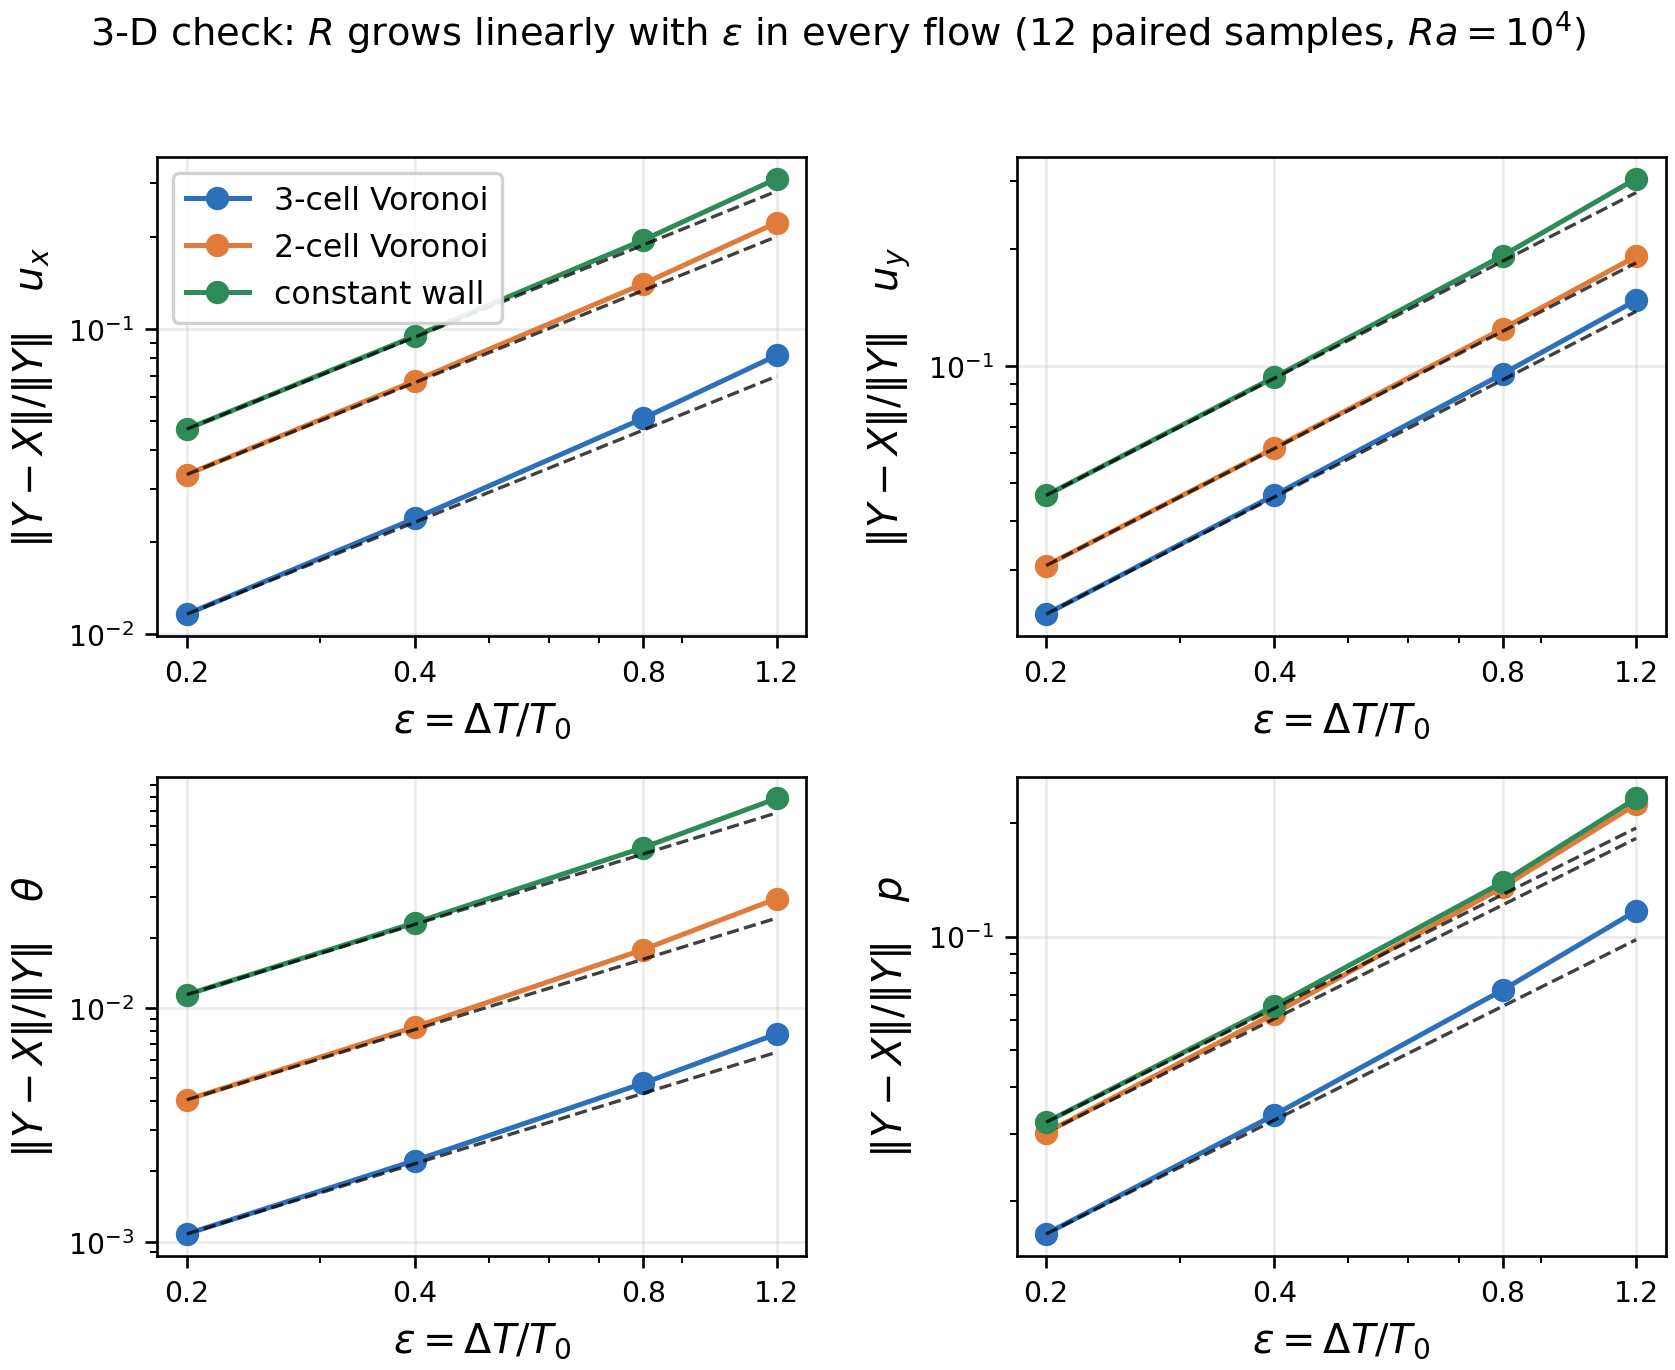
\includegraphics[width=0.95\textwidth]{fig9_3d.png}
\caption{The three-dimensional check in log--log coordinates for the two lower-Rayleigh-number
sets (24 paired samples), three wall types at $Ra=10^4$ and $3\times10^4$; the $Ra=10^5$ set is
tabulated in Table~\ref{tab:3d} and is not drawn. The vertical axis is $R=\|Y-X\|/\|Y\|$ in the channel labelled in
each panel. Filled symbols and solid lines: $Ra=10^4$ over five contrasts; open symbols and dashed
lines: $Ra=3\times10^4$ over three contrasts. Lines connect the samples, not the fitted laws, and
open symbols carry the colour of their wall type. The dotted line is a slope-one reference anchored
at the lowest $\varepsilon$ of the three-cell $Ra=10^4$ curve.}
\label{fig:3d}
\end{figure}

\section*{S10 Mesh independence, solver noise and the two-term fit}
\subsection*{Mesh independence}
At $Ra=10^5$ the same isothermal-wall check at $\varepsilon=1.2$ and $1.9$ gives a wall-$Nu$
change of $-0.15$ and $-0.36$ percentage points between $64^2$ and $128^2$ ($Nu_X$ itself moves by
$0.86\%$); the integral correction moves from $+0.87\%$ to $+0.73\%$ at $\varepsilon=1.2$ and from
$-1.81\%$ to $-2.16\%$ at $\varepsilon=1.9$. Across $Ra=10^4$, $10^5$ and $10^6$ the change between $64^2$ and $128^2$ is therefore at most
$0.38$ percentage points, and the sign and order of the integral correction are unchanged.

At $Ra=10^6$ the isothermal-wall pair was refined to $192^2$ and, at $\varepsilon=1.2$, to
$256^2$. At $\varepsilon=1.2$ the wall-$Nu$ correction falls from $+0.82\%$ at $64^2$ to $+0.56\%$
at $128^2$ and $+0.44\%$ at $256^2$, where eight temperature nodes span the thermal boundary layer.
The absolute Boussinesq value at $256^2$ is $Nu=8.793$, $0.37\%$ below the benchmark $8.825$ of
Le Qu\'er\'e \citep{lequere1991}; the $64^2$ and $128^2$ values are $8.563$ and $8.759$, so the
grid sequence approaches the benchmark.
At $\varepsilon=1.9$ it moves from $-1.50\%$ at $64^2$ to $-1.88\%$ at $128^2$ and $-2.10\%$ at
$192^2$. Both sequences are still moving at the finest mesh, by $0.12$ and $0.22$ percentage
points per step, so the integral values carry a resolution uncertainty of that order; the sign and
the order of magnitude do not change. The $\varepsilon=1.9$ pair at $256^2$ did not reach the
steady tolerance: at pseudo-time step $0.05$ it ran for $4.5$\,h and stopped at a relative change of
$4\times10^{-6}$ per step against the $10^{-6}$ target, and the step $0.025$ retry did not
converge either.




\subsection*{Solver noise}



\begin{itemize}
\item Convergence quality over 600 samples (compressible member): median relative change
$3.75\times10^{-6}$, p90 $1.09\times10^{-4}$, worst $7.04\times10^{-4}$.
\item Dropping the 65 samples with relative change $>10^{-4}$ changes the linear $u_x$ fit from
$0.1809\varepsilon-0.0212$ to $0.1813\varepsilon-0.0221$---unchanged. The negative intercept is a
property of this linear fit; the power-law fit of Table~\ref{tab:law} has an intercept consistent
with zero.
\item Re-running the 10 worst samples with \path{steady_tol} tightened from $10^{-6}$ to
$10^{-8}$ leaves the solution bit-identical ($|\Delta Y|/|Y|=0$). The reason is
structural: the compressible march terminates on the zero-iteration guard, not on
\path{steady_tol}, so the residual reported is the fixed-point residual of the discrete solution,
not unfinished iteration.
\end{itemize}

\subsection*{A two-term fit} The same low-$\varepsilon$ pairs allow a stronger
data-driven baseline: fit $\mathcal{P}(\varepsilon)=P+\varepsilon Q$ on $\varepsilon=0.4,0.8,1.2$ for each
configuration and predict $X+\varepsilon P+\varepsilon^2Q$. At $\varepsilon=1.6$ this gives
$3.3$/$3.9$/$0.4$/$3.8\%$ and at $\varepsilon=1.9$ $11.4$/$13.9$/$1.7$/$13.8\%$
($u_x/u_y/\theta/p$), against $14$/$15$/$1.4$/$15\%$ and $24$/$27$/$3.0$/$28\%$ for the
first-order response. That is the same order as the network's $9.4$/$10.6$/$1.4$/$11.3\%$,
averaged over the extrapolation split; the two are not evaluated on the same samples. The two-term fit is available only when paired
low-$\varepsilon$ data exist for the target flow. The public-data problem of Sec.~\ref{sec:public}
has no such pairs at the target contrast; there a single-$\varepsilon$ data set is all that exists,
and the prior---not a quadratic fit---is what makes it reusable.

\section*{S11 Per-sample field--$Nu$ statistics within a family}

Table~\ref{tab:ownfieldnu} repeats the per-sample comparison of Sec.~\ref{sec:headline} inside
the random-wall family. A prior is trained on 400 of our 600 samples and evaluated on the
held-out 200-sample split; 22 of those samples lie at $\varepsilon=1.1$--$1.3$ and form the
comparison set below. The field error is the per-sample median relative $L_2$; the $Nu$ error is
the both-wall integral error. The wall-flux penalty is the same one used for the public-data
model. The pattern is the same as in the classical cavity: a field error below $1\%$ coexists
with a $Nu$ error above $2\%$ in $66\%$ of the 22 samples, and the wall-flux penalty removes
most of the bias.

\begin{table}[htbp]
\centering
\footnotesize
\setlength{\tabcolsep}{4pt}
\caption{Per-sample statistics at $\varepsilon\approx1.2$. Classical cavity: 200
held-out public samples, public-data model of Sec.~\ref{sec:headline} (range across models).
Random walls: 22 held-out samples at $\varepsilon=1.1$--$1.3$, drawn from the 200-sample
split; prior trained on the other 400. The last column is the mean local wall-flux error.}
\label{tab:ownfieldnu}
\begin{tabular}{@{}llcccc@{}}
\toprule
family & model & $T$ median & $Nu$ median & $T<1\%$, $Nu>2\%$ & local\\
\midrule
classical cavity & prior & 0.09\% & 1.4--2.9\% & 23--82\% & 4.5\%\\
classical cavity & prior + wall-flux & 0.10\% & 0.01\% & 0\% & 0.08\%\\
random walls & prior & 0.47\% & 4.04\% & 66\% & 4.94\%\\
random walls & prior + wall-flux & 0.49\% & 0.58\% & 16\% & 1.14\%\\
\bottomrule
\end{tabular}
\end{table}


\end{document}
